\section{Laplace-Transformation (LPT)}
	Hintransformation - Analyse:
	\[
		 \mathcal{L}\left\{ x(t) \right\} = \boxed{ \underline{X}(s) = \int_0^\infty x(t) \cdot e^{-st} dt }
	\]
	Rücktransformation - Synthese:
	\[
		 \mathcal{L}^{-1}\left\{ \underline{X}(s) \right\} = x(t) =  \frac{1}{2\pi j}\int_{\sigma-j\infty}^{\sigma+j\infty} \underline{X}(s) \cdot e^{-st} ds
	\]
LPT mit Partialbruchzerlegung (PBZ) + Tabelle.

\normalsize
\subsection{LTI-Systeme im Bildbereich (BB)}
$x(t)=h(t)=0$ für $t<0$: Rechtsseitige (\textbf{kausale}) Signale!
\begin{center}
	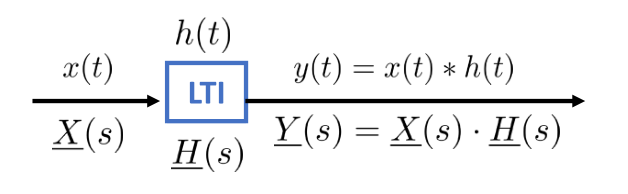
\includegraphics[width=0.6\columnwidth]{Bilder/LTI_Systeme_im_Bildbereich.png}
\end{center}
LTI-Systeme im Bildbereich sind \textbf{immer} kausal!

\subsection{Impuls- und Sprungantwort im BB}
Impulsantwort:
\[
h(t)\ \laplace\ \underline{H}(s)
\]
Sprungantwort:
\[
g(t) = \int_0^t h(\tau) d\tau \quad \laplace\ \quad \boxed{\underline{G}(s) = \frac{\underline{H}(s)}{s}}
\]

\subsection{Zusammenhang LPT $\leftrightarrow$ FT}
\begin{itemize}
		\item Konvergenzbereich (Kb): Halbebene rechts vom am \underline{weitesten} rechts liegenden Pol.
	\item Wenn $\omega$-Achse $\in$ Kb: FT von $\underline{X}(s)$ existiert:
	\[
	\mathcal{F}\{x(t)\} = X(\omega) = X(s) \big|_{s=j\omega} = \mathcal{L}\{x(t)\} \big|_{s=j\omega}
	\]
\end{itemize}

\subsection{P/N-Diagramm: Systemeigenschaften}
\begin{itemize}
	\item \textbf{Stabilität}: \textbf{Alle} Pole von $\underline{H}(s)$ liegen links der $\omega$-Achse. Bei Ü-Fkt.:  Nennergrad $\ge$ Zählergrad.
	\item Minimalphasiges System: Alle Nullstellen liegen links der $\omega$-Achse.
\end{itemize}
\subsection{Partialbruchzerlegung (PBZ)}
Für die inverse bzw. Rücktransformation in Zeitbereich. Beispiele siehe Papula FS. S.157f.
\begin{itemize}
	\item Einfache Polstellen:
		\begin{align*}
		\underline{X}(s) &= \frac{\underline{Z}(s)}{\underline{N}(s)} = \sum_{n=1}^{N} \frac{A_n}{(s - p_n)}
	\end{align*}
	\item Doppelte/k-fache Polstellen:
	\begin{align*}
			\underline{X}(s) &= \frac{\underline{Z}(s)}{\underline{N}(s)} = \frac{\underline{Z}(s)}{(s - p_n)^k} \\
			&= \frac{A_1}{s - p_{n}} + \frac{A_2}{(s - p_{n})^2} + \cdots + \frac{A_k}{(s - p_{n})^k}
	\end{align*}
	\item \textbf{Komplexe} Polstellen:
		\begin{align*}
		\underline{X}(s) = \frac{\underline{Z}(s)}{\underline{N}(s)} 
		&= \frac{\underline{Z}(s)}{(s -p_{1})(s - p_{1}^*)}\\
		&= \frac{B \, s+C}{(s -p_{1})(s - p_{1}^*)}\\ &= \frac{B \, s+C}{(s -jp_{1})(s +jp_{1})}
	\end{align*}
\end{itemize}
\small \textbf{Beachte}: Wenn Zählergrad $>$ Nennergrad, muss vor der PBZ eine \textbf{Polynomdivision} durchgeführt werden!
\normalsize
%\subsection{Systemantwort von LTI Systemen}
%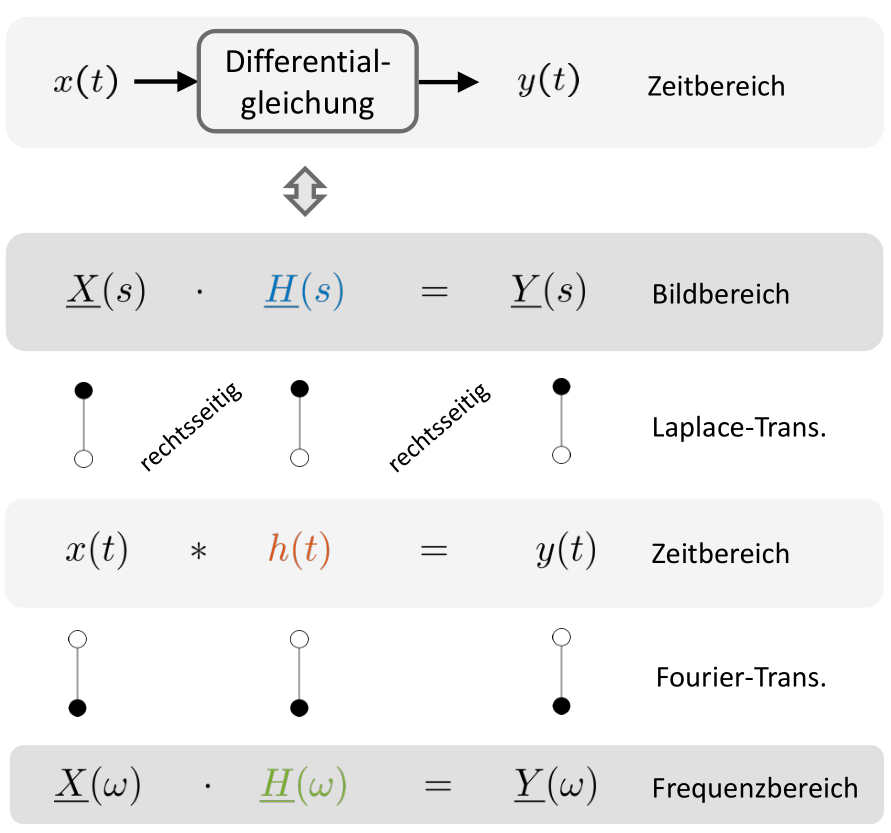
\includegraphics[width=0.98\columnwidth]{Bilder/LTI_Systemantworten.png}
%\clearpage
\subsection{Eigenschaften der LPT}
\renewcommand{\arraystretch}{1.7}
\begin{tabularx}{\columnwidth}{|X|X|X|}
	\hline
	& $\mathbf{x(t)}$ & \underline{$\mathbf{X}$}$\mathbf{(s)}$\\
	\hline Linearität & $a x_{1}(t)+b x_{2}(t)$ & $a \underline{X}_{1}(s)+b\underline{X}_{2}(s)$ \\
	\hline Skalierung $t$ & $x(at)$ & $\frac{1}{a} \underline{X}(\frac{s}{a})$ \\
	\hline Skalierung $s$ & $\frac{1}{a} x(\frac{t}{a})$ & $\underline{X}(as)$ \\
	\hline Verschiebung	& $x(t-t_0)$ & $e^{-s \cdot t_0} \underline{X}(s)$ \\
	\hline Modulation & $e^{at} \, x(t)$ & $\underline{X} (s-a)$ \\
	\hline Multiplikation & $t \cdot x(t) $ & $-\frac{d}{d s} \underline{X}(s)$ \\
	\hline Faltung & $x_{1}(t) * x_{2}(t) $ & $ \underline{X}_{1}(s) \cdot \underline{X}_{2}(s)$ \\
	\hline Differentiation $t$ & $ \frac{d}{dt} x(t) $ & $ s\cdot \underline{X}(s)-x(0)$ \\
	\hline Integration $t$ & $\int_{0}^{t} x(\tau) \, d\tau $ & $ \frac{1}{s} \underline{X}(s)$ \\
	\hline Integration $s$ & $\frac{1}{t} \cdot x(t) $ & $ \int_{s}^{\infty} \underline{X}(s) \, ds$ \\
	\hline
\end{tabularx}
\clearpage
\end{multicols*}
\begin{table}[h!]
	\subsection{Korrespondenzen der LPT}
	\renewcommand{\arraystretch}{1.7}
\begin{minipage}[t]{0.5\columnwidth}
	\begin{tabularx}{\columnwidth}{|l|l|X|}
		\hline
		Nr. & $\mathbf{x(t)}$ für $t \geq 0$ & $\mathbf{\underline{X}(s)}$ \\
		\hline 
		10 & 1 & $\frac{1}{s}$ \\
		\hline
		11 & $t$ & $\frac{1}{s^2}$ \\
		\hline
		12 & $\frac{t^n}{n!}$ & $\frac{1}{s^{n+1}}$ \\
		\hline
		13 & $\mathrm{e}^{-a t}$ & $\frac{1}{s+a}$ \\
		\hline
		14 & $\frac{1}{a} \cdot\left(1-\mathrm{e}^{-a t}\right)$ & $\frac{1}{s(s+a)}$ \\
		\hline
		15 & $\sin (a t)$ & $\frac{a}{s^2+a^2}$ \\
		\hline
		16 & $\sinh (a t)$ & $\frac{a}{s^2-a^2}$ \\
		\hline
		17 & $\cos (a t)$ & $\frac{s}{s^2+a^2}$\\
		\hline
		18 & $\cosh (a t)$ & $\frac{s}{s^2-a^2}$\\
		\hline
		19 & $t \cdot \mathrm{e}^{-a t}$ & $\frac{1}{(s+a)^2}$\\
		\hline
		20 & $(1-a t) \cdot \mathrm{e}^{-a t}$ & $\frac{s}{(s+a)^2}$\\
		\hline 21 & $\frac{1}{a^2} \cdot\left[1-(1+a t) \cdot \mathrm{e}^{-a t}\right]$ &
		$\frac{1}{s(s+a)^2}$ \\
		\hline 22 & 
		$\frac{t^2}{2} \cdot \mathrm{e}^{-a t}$ & 	$\frac{1}{(s+a)^3}$	\\
		\hline 23 & 	$\frac{1}{a^2} \cdot(1-\cos a t)$ & 	$\frac{1}{s\left(s^2+a^2\right)}$ \\
		\hline 24 & 	$\frac{1}{a^2} \cdot(\cosh a t-1)$ & 	$\frac{1}{s\left(s^2-a^2\right)}$\\
		\hline 25 & 	$\frac{1}{a^2} \cdot\left[a t-1+\mathrm{e}^{-a t}\right]$ & $\frac{1}{s^2(s+a)}$ \\
		\hline 26 & 	$\frac{\mathrm{e}^{-a t}-\mathrm{e}^{-b t}}{b-a}$& 	$\frac{1}{(s+a) \cdot(s+b)}$\\
		\hline 27 & 	$\frac{a \cdot \mathrm{e}^{-a t}-b \cdot \mathrm{e}^{-b t}}{a-b}$ & 	$\frac{s}{(s+a) \cdot(s+b)}$ \\
		\hline
	\end{tabularx}
\end{minipage}
\begin{minipage}{0.5\columnwidth}
\begin{tabularx}{\columnwidth}{|l|l|X|}
			\hline
	Nr. & $\mathbf{x(t)}$ für $t \geq 0$ & $\mathbf{\underline{X}(s)}$ \\
			\hline 28 & 
	$\frac{1}{a b}+\frac{b \cdot \mathrm{e}^{-a t}-a \cdot \mathrm{e}^{-b t}}{a b \cdot(a-b)}$
	& 
	$\frac{1}{s(s+a)(s+b)}$
	\\	
		\hline 29 & 
		$\frac{\mathrm{e}^{-a t}+[(a-b) t-1] \cdot \mathrm{e}^{-b t}}{(a-b)^2}$
		& 
		$\frac{1}{(s+a)(s+b)^2}$
		\\
		\hline 30 & 
		$\frac{[a-b(a-b) t] \cdot \mathrm{e}^{-b t}-a \cdot \mathrm{e}^{-a t}}{(a-b)^2}$
		& 
		$\frac{s}{(s+a)(s+b)^2}$
		\\
		\hline 31 & 
		$\frac{(b-c) \cdot \mathrm{e}^{-a t}+(c-a) \cdot \mathrm{e}^{-b t}+(a-b) \cdot \mathrm{e}^{-c t}}{(b-a)(c-a)(b-c)}$ & 
		$\frac{1}{(s+a)(s+b)(s+c)}$ \\
		\hline 32 & 
		$\frac{a(b-c) \cdot \mathrm{e}^{-a t}+b(c-a) \cdot \mathrm{e}^{-b t}+c(a-b) \cdot \mathrm{e}^{-c t}}{(b-a)(c-b)(c-a)}$ & $\frac{s}{(s+a)(s+b)(s+c)}$ \\
		\hline 33 & $\frac{1}{2 \omega^3} \cdot(\sin \omega t-\omega t \cdot \cos \omega t)$ & $\frac{1}{\left(s^2+\omega^2\right)^2}$ \\
		\hline 34 & $\frac{t}{2 \omega} \cdot \sin \omega t$ & $\frac{s}{\left(s^2+\omega^2\right)^2}$ \\
		\hline 35 & $\frac{1}{2 \omega} \cdot(\sin \omega t+\omega t \cdot \cos \omega t)$ & $\frac{s^2}{\left(s^2+\omega^2\right)^2}$ \\
		\hline 36 & $\sin ^2(\omega t)$ & 
		$\frac{2 \omega^2}{s\left(s^2+4 \omega^2\right)}$ \\
		\hline 37 & $\cos ^2(\omega t)$ & 
		$\frac{s^2+2 \omega^2}{s\left(s^2+4 \omega^2\right)}$ \\
		\hline 38 & $\cos (\omega t+\psi)$ & 
		$\frac{s \cos \psi-\omega \sin \psi}{s^2+\omega^2}$ \\
		\hline 39 & $\sin (\omega t+\psi)$ & $\frac{s \sin \psi+\omega \cos \psi}{s^2+\omega^2}$ \\
		\hline 40 & $\mathrm{e}^{-a t} \cdot \cos (\omega t)$ & 
		$\frac{s+a}{(s+a)^2+\omega^2}$ \\
		\hline 41 & $\mathrm{e}^{-a t} \cdot \sin (\omega t)$ & 
		$\frac{\omega}{(s+a)^2+\omega^2}$ \\
		\hline 42 & $\mathrm{e}^{-a t} \cdot \cos (\omega t+\psi)$ & 
		$\frac{(s+a) \cos \psi-\omega \sin \psi}{(s+a)^2+\omega^2}$ \\
		\hline 43 & 
		$\frac{a \cos \omega t+\omega \sin \omega t-a \cdot \mathrm{e}^{-a t}}{a^2+\omega^2}$ &
		$\frac{s}{s^2+\omega^2} \cdot \frac{1}{s+a}$\\
		\hline 44 & 
		$\frac{a \sin \omega t-\omega \cos \omega t+\omega \cdot \mathrm{e}^{-a t}}{a^2+\omega^2}$ & 
		$\frac{\omega}{s^2+\omega^2} \cdot \frac{1}{s+a}$ \\
		\hline 45 & 
		$\frac{\cos (\omega t+\psi-\gamma)-\cos (\psi-\gamma) \cdot \mathrm{e}^{-a t}}{\sqrt{a^2+\omega^2}}$ & 
		$\frac{s \cos \psi-\omega \sin \psi}{\left(s^2+\omega^2\right) \cdot(s+a)}$ \\
		\hline
	\end{tabularx}
\end{minipage}
\end{table}
\noindent
\begin{minipage}{0.68\columnwidth}
	\renewcommand{\arraystretch}{1.7}
	\begin{tabularx}{\columnwidth}{|l|c|X|}
		\hline Nr  & $\mathbf{x(t)}$ für $t \geq 0$ & $\mathbf{\underline{X}(s)}$ \\
		\hline 46  & \begin{tabular}{l}
			\begin{tabular}{l}
				$a^2>b^2: \frac{1}{2 W} \cdot\left(\mathrm{e}^{\lambda_1 t}-\mathrm{e}^{\lambda_2 t}\right)$ \\
				$a^2=b^2: t \cdot \mathrm{e}^{-a t}$ \\
				$a^2<b^2: \frac{1}{\omega_d} \cdot \mathrm{e}^{-a t} \cdot \sin \omega_{\mathrm{d}} t$
			\end{tabular}
		\end{tabular} & $\dfrac{1}{s^2+2 a s+b^2}$\\
		\hline 47   & \begin{tabular}{l}
			\begin{tabular}{l}
				$a^2>b^2: \frac{1}{2 W} \cdot\left(\lambda_1 \mathrm{e}^{\lambda_1 t}-\lambda_2 \mathrm{e}^{\lambda_2 t}\right)$ \\
				$a^2=b^2:(1-a t) \cdot \mathrm{e}^{-a t}$ \\
				$a^2<b^2:\left(\cos \omega_{\mathrm{d}} t-\frac{a}{\omega_{\mathrm{d}}} \cdot \sin \omega_{\mathrm{d}} t\right) \cdot \mathrm{e}^{-a t}$
			\end{tabular}
		\end{tabular} & 
			$\dfrac{s}{s^2+2 a s+b^2}$ \\
		\hline 48 & \begin{tabular}{l}
			\begin{tabular}{l}
				$a^2>b^2: \frac{1}{b^2}\left(1+\frac{\lambda_2}{2 W} \cdot \mathrm{e}^{\lambda_1 t}-\frac{\lambda_1}{2 W} \cdot \mathrm{e}^{\lambda_2 t}\right)$ \\
				$a^2=b^2: \frac{1}{a^2}\left[1-(1+a t) \cdot \mathrm{e}^{-a t}\right]$ \\
				$a^2<b^2: \frac{1}{b^2}\left[1-\left(\cos \omega_{\mathrm{d}} t+\frac{a}{\omega_{\mathrm{d}}} \cdot \sin \omega_{\mathrm{d}} t\right) \cdot \mathrm{e}^{-a t}\right]$
			\end{tabular}
		\end{tabular} & 
			$\dfrac{1}{s\left(s^2+2 a s+b^2\right)}$
		 \\
		\hline 49 &
			\begin{tabular}{l}
				$a^2>b^2: \frac{\cos (\omega_0 t+\varphi)+k_1 \cdot \mathrm{e}^{-\lambda_1 t}+k_2 \cdot \mathrm{e}^{-\lambda_2 t}}{\sqrt{x^2+y^2}}$ \\
				$a^2=b^2: \frac{\cos (\omega_0 t+\varphi)+(z t-\cos \varphi) \cdot \mathrm{e}^{-a t}}{\sqrt{x^2+y^2}}$ \\
				$a^2<b^2: \frac{\cos (\omega_0 t+\varphi)-k \cdot \cos \left(\omega_{\mathrm{d}} t+\beta\right) \cdot \mathrm{e}^{-a t}}{\sqrt{x^2+y^2}}$
			\end{tabular}
		 & 
			$\frac{s \cos \psi-\omega \sin \psi}{\left(s^2+\omega^2\right) \cdot\left(s^2+2 a s+b^2\right)}$
		\\
		\hline
	\end{tabularx}
\end{minipage}
\begin{minipage}{0.33\columnwidth}
{\centering
\begin{itemize}
	\item Aperiodischer Kriechfall:\\
	$a^2>b^2 \, \leftrightarrow \, \vartheta>1$
	
	\item Aperiodischer \textbf{Grenzfall:}\\
	$a^2=b^2 \, \leftrightarrow \, \vartheta=1$
	
	\item Periodischer Schwingfall:\\
	$a^2<b^2 \, \leftrightarrow \, 0<\vartheta<1$
	
	\item Abklingkonstante:\\
	$a=\delta =\frac{\vartheta}{T} = \frac{R}{2L}$
	
	\item Resonanz-Kreisfrequenz:\\
	$b=\omega_0=\frac{1}{T} =\frac{1}{\sqrt{LC}}$
	
	\item Eigen-Kreisfrequenz:\\
	$\omega_d = \sqrt{b^2-a^2}$ \\
	wenn $\vartheta=0 \rightarrow \omega_0 = \omega_d$
	
	\item Dämpfungsgrad:\\
	$D = \vartheta = \frac{\delta}{\omega_0} = \frac{a}{b}$
\end{itemize} 
}
\end{minipage}
$\arraycolsep=1.7pt\def\arraystretch{1.7}
\begin{array}{cccc}
	\lambda_{1,2}=-a\pm W = -a\pm j\omega_d & \quad W=\sqrt{a^2-b^2}=j\omega_d & \quad x=b^2-\omega^2$ \qquad $y=2a\omega & \quad z=\omega \sin\varphi - a \cos \varphi\\
	\varphi=\arctan\dfrac{x\sin\varphi-y\cos\varphi}{y\sin\varphi+x\cos\varphi} & k=\dfrac{\cos\varphi}{\cos\beta} & k_1=\dfrac{\lambda_2\cos\varphi-\omega\sin\varphi}{2W} & k_2=\dfrac{\omega\sin\varphi-\lambda_1\cos\varphi}{2W}
\end{array}$\\
\vspace{5em}
$\beta=\arctan\frac{z}{\omega_d \, \cos\varphi}$
\newpage
\begin{multicols*}{2}
%\begin{mdframed}[style=exercise,nobreak=false]
%	\begin{itemize}
%		\item \textbf{Linearität}
%		      \[
%			      \alpha x_1(t) + \beta x_2(t) \ \laplace\  \alpha \underline{X}_1(t) + \beta \underline{X}_2(t)
%		      \]
%		      \vspace{-1.5em}
%		\item \textbf{Skalierung im Zeitbereich}
%		      \[
%			      x(\alpha t) \ \laplace\  \frac{1}{\alpha} \underline{X}\left(\frac{s}{\alpha}\right) \qquad \color{red}{\alpha > 0}
%		      \]
%		      \vspace{-1.5em}
%		\item \textbf{Skalierung im Bildbereich}
%		      \[
%			      \frac{1}{\alpha}x\left(\frac{t}{\alpha}\right)\ \laplace\ \underline{X}(\alpha s) \qquad \color{red}{\alpha > 0}
%		      \]
%		      \vspace{-1.5em}
%		\item \textbf{Verschiebung im Zeitbereich}
%		      \[
%			      x(t-t_0)\ \laplace\ e^{-st_0} \underline{X}(s) \qquad \color{red}{t_0 > 0}
%		      \]
%		      \vspace{-1.5em}
%		\item \textbf{Verschiebung im Bildbereich - Modulation}
%		      \[
%			      e^{at}x(t) \ \laplace\ \underline{X}(s-a)
%		      \]
%		      \vspace{-1.5em}
%		\item \textbf{Faltung}
%		      \[
%			      x_1(t)*x_2(t) \ \laplace\ \underline{X}_1(s)\cdot \underline{X}_2(s)
%		      \]
%		      \vspace{-1.5em}
%		\item \textbf{Differentiation im Zeitbereich}
%		      \[
%			      \frac{d}{dt}x(t) \ \laplace\ s\cdot\underline{X}(s)\color{red}{-x(0^+)}
%		      \]
%		      \vspace{-1.5em}
%		\item \textbf{Differentiation im Bildbereich}
%		      \[
%			      t\cdot x(t) \ \laplace\ -\frac{d}{ds}\underline{X}(s)
%		      \]
%		      \vspace{-1.5em}
%		\item \textbf{Integration im Zeitbereich}
%		      \[
%			      \int_0^t x(\tau)d\tau \ \laplace\ \frac{1}{s}\underline{X}(s)
%		      \]
%		      \vspace{-1.5em}
%		\item \textbf{Integration im Bildbereich}
%		      \[
%			      \frac{1}{t}x(t) \ \laplace\ \int_s^\infty\underline{X}(s)ds
%		      \]
%	\end{itemize}
%\end{mdframed}
%\subsubsection{Rücktransformation rationaler Funktionen}
%\footnotesize
%Partialbruchzerlegung: Siehe papula nach S.157
